\section{Δεύτερη Φάση Πειραμάτων}
\label{sec:experiments_phase2}

Η μεταγλώττιση των δικτύων AlexNet και VGG16 απαιτεί περισσότερη
μνήμη από αυτή που διαθέτει το ενσωματωμένο σύστημα Jetson TK1 (1888MB).
Το πρόβλημα αυτό το αντιμετωπίστηκε προσθέτοντας 1GB μνήμη
\emph{Swap}\footnote{Δημιουργία αρχείου μνήμης swap: \url{http://www.jetsonhacks.com/2014/10/04/creating-swapfile-ubuntu-nvidia-jetson-tk1/}}.

%%----------------------------------------------------------------------------

\subsection{AlexNet}

Οι παράμετροι των πειραμάτων είναι οι εξής:
\begin{itemize}
  \item{Αριθμός επαναλήψεων: 100}
  \item{Υπολογιστική μονάδα:}
    \begin{itemize}
      \item{CPU: Αριθμός Νημάτων (1, 2, 4, 8)}
      \item{GPU: Με και χωρίς εκ των προτέρων δέσμευση μνήμης}
    \end{itemize}
\end{itemize}

\begin{figure}[H]
  \centering
  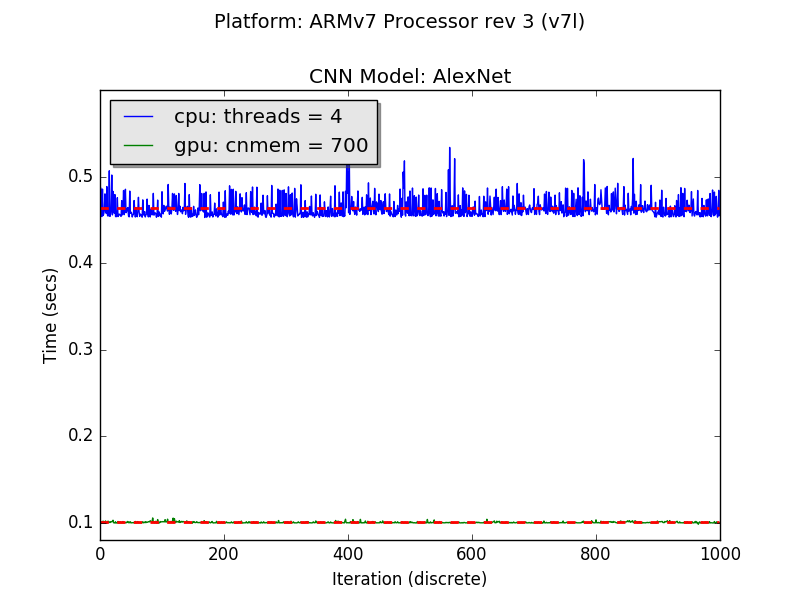
\includegraphics[width=0.8\textwidth]{./images/chapter6/benchmark_alexnet_jetson.png}
  \caption[Χρόνoι εκτέλεσης για το δίκτυο AlexNet στο Jetson TK1]{Χρόνoι εκτέλεσης για το δίκτυο AlexNet στο Jetson TK1}
  \label{fig:alexnet_results_jetson}
\end{figure}

Στον \autoref{tab:alexnet_jetson} παρουσιάζονται τα συγκριτικά αποτελέσματα της
εκτέλεσης τόσο στην μονάδα CPU (με μεταβλητό αριθμό νημάτων), όσο και στην
GPU (με και χωρίς εκ-των προτέρων δέσμευση μνήμης).

\begin{table}[H]
  \begin{center}
    \caption{Μετρήσεις πειραμάτων για το δίκτυο AlexNet στο Jetson TK1}
    \label{tab:alexnet_jetson}
    \small
    \begin{tabular}[center]{ | c | c | c | c | c | }
      \hline
      \rowcolor{Gray}
      Υπολ. Μονάδα & \# νημάτων & cnmem & Χρόνος εκτέλεσης (sec) & Κατ. Ισχύος (Watts) \\
      \hline
      CPU & 1 & N/A & 0.62 & 6.318\\
      CPU & 2 & N/A & 0.4845 & 8.019\\
      CPU & 4 & N/A & 0.4634 & 10.692\\
      CPU & 8 & N/A & 0.4646 & 10.692\\
      GPU & N/A & None & 0.1049 & 8.5\\
      GPU & N/A & 700MB & 0.1 & 8.5\\
      \hline
    \end{tabular}
  \end{center}
\end{table}


%%----------------------------------------------------------------------------

\subsection{VGG16}

Οι παράμετροι των πειραμάτων είναι οι εξής:
\begin{itemize}
  \item{Αριθμός επαναλήψεων: 100}
  \item{Υπολογιστική μονάδα:}
    \begin{itemize}
      \item{CPU: Αριθμός Νημάτων (1, 2, 4, 8)}
      \item{GPU: Με και χωρίς εκ των προτέρων δέσμευση μνήμης (cnmem)}
    \end{itemize}
\end{itemize}

Στον \autoref{tab:vgg16_jetson} παρουσιάζονται τα συγκριτικά αποτελέσματα της
εκτέλεσης τόσο στην μονάδα CPU (με μεταβλητό αριθμό νημάτων), όσο και στην
GPU (με και χωρίς εκ-των προτέρων δέσμευση μνήμης).

\begin{table}[H]
  \begin{center}
    \caption{Μετρήσεις πειραμάτων για το δίκτυο VGG16 στο Jetson TK1}
    \label{tab:vgg16_jetson}
    \small
    \begin{tabular}[center]{ | c | c | c | c | c | }
      \hline
      \rowcolor{Gray}
      Υπολ. Μονάδα & \# νημάτων & cnmem & Χρόνος εκτέλεσης (sec) & Κατ. Ισχύος (Watts) \\
      \hline
      CPU & 1 & N/A & 9.431 & 6.318 \\
      CPU & 2 & N/A & 5.4476 &  8.748\\
      CPU & 4 & N/A & 3.6224 & 13.122\\
      CPU & 8 & N/A & 3.6308 & 13.122\\
      GPU & N/A & None & 0.6983 & 11.907\\
      GPU & N/A & 720MB & 0.5761 & 11.907\\
      \hline
    \end{tabular}
  \end{center}
\end{table}

Παρατηρούμε ότι η εκτέλεση στην μονάδα GPU είναι 5.187 φορές πιο
γρήγορη (χωρίς εκ-των προτέρων δέσμευση μνήμης).
Επίσης, με εκ-των-προτέρων δέσμευση μνήμης για την μονάδα GPU, ο χρόνος εκτέλεσης μειώνεται ακόμη
περισσότερο (περίπου 120ms).

Στο \autoref{fig:vgg16_results_jetson} βλέπουμε το διάγραμμα
των χρόνων εκτέλεσης στην μονάδα CPU με χρήση τεσσάρων νημάτων και στην μονάδα
GPU με εκ-των-προτέρων δέσμευση 720MB μνήμης.

\begin{figure}[!ht]
  \centering
  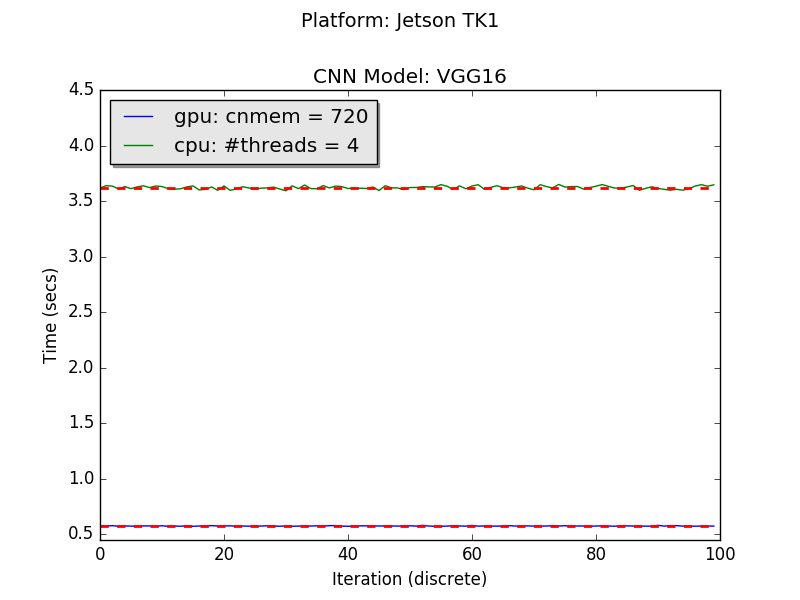
\includegraphics[width=0.8\textwidth]{./images/chapter6/benchmark_vgg16_jetson.png}
  \caption[Χρόνoι εκτέλεσης για το δίκτυο VGG16 στο Jetson TK1]{Χρόνoι εκτέλεσης για το δίκτυο VGG16 στο Jetson TK1}
  \label{fig:vgg16_results_jetson}
\end{figure}


%%----------------------------------------------------------------------------

\subsection{Tiny-YOLO}

Οι παράμετροι των πειραμάτων είναι οι εξής:
\begin{itemize}
  \item{Αριθμός επαναλήψεων: 1000}
  \item{Υπολογιστική μονάδα:}
    \begin{itemize}
      \item{CPU: Αριθμός Νημάτων (1, 2, 4, 8)}
      \item{GPU: Με και χωρίς εκ των προτέρων δέσμευση μνήμης (cnmem)}
    \end{itemize}
\end{itemize}

\begin{table}[!ht]
  \begin{center}
    \caption{Μετρήσεις πειραμάτων για το δίκτυο Tiny-YOLO στο Jetson TK1}
    \label{tab:yolo_jetson}
    \small
    \begin{tabular}[center]{ | c | c | c | c | c | }
      \hline
      \rowcolor{Gray}
      Υπολ. Μονάδα & \# νημάτων & cnmem & Χρόνος εκτέλεσης (sec) & Κατ. Ισχύος (Watts) \\
      \hline
      CPU & 1 & N/A & 1.5902 & 6.318\\
      CPU & 2 & N/A & 1.0276 & 8.504\\
      CPU & 4 & N/A & 0.8137 & 11.9\\
      CPU & 8 & N/A & 0.8126 & 11.9\\
      GPU & N/A & None & 0.5543 & 8\\
      GPU & N/A & 400MB & 0.3872 & 8\\
      \hline
    \end{tabular}
  \end{center}
\end{table}

\begin{figure}[!ht]
  \centering
  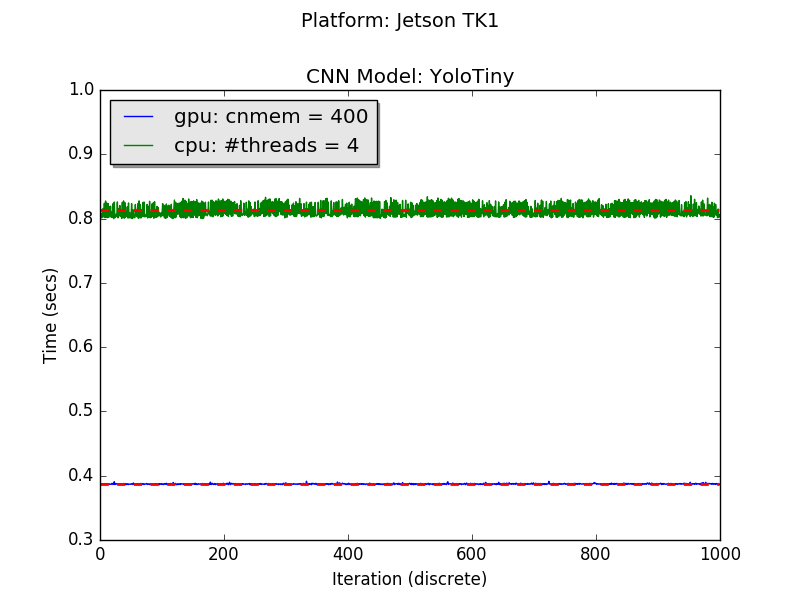
\includegraphics[width=0.8\textwidth]{./images/chapter6/benchmark_yolotiny_jetson.png}
  \caption[Χρόνoι εκτέλεσης για το δίκτυο Tiny-YOLO στο Jetson TK1]{Χρόνοι εκτέλεσης για το δίκτυο Tiny-YOLO στο Jetson TK1}
  \label{fig:yolotiny_results_jetson}
\end{figure}

Ο χρόνος εκτέλεσης της αντίστοιχης υλοποίησης της ερευνητικής ομάδας που
σχεδίασε το δίκτυο Tiny-YOLO μετρήθηκε, για την μονάδα CPU του Tegra K1,
στα 3.475 δευτερόλεπτα (τέσσερις φορές πιο αργό από την υλοποίηση
μας).
Η μέτρηση του χρόνου εκτέλεση της αντίστοιχης
υλοποίησης στην μονάδα GPU ήταν αδύνατη. Η εκτέλεση στην μονάδα GPU
απαιτούσε περισσότερη μνήμη από όση η πλατφόρμα Jetson TK1 διαθέτει και έτσι
το εκτελέσιμο τερματίζει με σφάλμα \emph{CUDA Error: out of memory}.
Ο λόγος που αυτό συμβαίνει μόνο στην περίπτωση εκτέλεσης στην μονάδα GPU
δεν είναι εμφανές. Πιθανόν να σφάλμα τύπου διαρροής μνήμης (memory leak).


